%
% teil3.tex -- Beispiel-File für Teil 3
%
% (c) 2020 Prof Dr Andreas Müller, Hochschule Rapperswil
%
% !TEX root = ../../buch.tex
% !TEX encoding = UTF-8
%
\section{Helmholtz-Zerlegung in der Akustik
\label{helmholtz:section:Helmholtz_Zerlegung_Akustik}}
\kopfrechts{Helmholtz-Zerlegung in der Akustik}


\subsection{Zerlegung des Schallschnellefeldes
\label{helmholtz:subsection:Zerlegung_Schallschnelle}}
Angewendet auf das Schallschnellefeld $\boldsymbol{u}$ können wir
dieses wie folgt zerlegen:
\begin{equation}
\underbrace{\boldsymbol{u}}_{\displaystyle\text{Schallschnellefeld}}
=
\underbrace{-\nabla \Phi}_{\displaystyle\text{irrotationaler~Anteil}}
+
\underbrace{\nabla \times \boldsymbol{\Psi}}_{\displaystyle\text{solenoidaler~Anteil}}.
\end{equation}
Die physikalische Interpretation der Komponenten des Schallschnellefeldes
lässt sich wie folgt beschreiben:
 
\begin{itemize}
\item Der irrotationale Anteil $-\nabla \Phi$ ist wirbelfrei, da die
Rotation verschwindet.
\begin{itemize}
\item Dieser Anteil hat keine Rotation: $\nabla \times (-\nabla \Phi) = 0$.
\item Die Feldlinien verlaufen strahlenförmig von Quellen zu Senken.
\end{itemize}
 
\item Der solenoidale Anteil $\nabla \times \boldsymbol{\Psi}$ hat gemäss
der Definition immer Divergenz null und wird auch quellenfrei genannt.
\begin{itemize}
\item Dieser Anteil hat keine Divergenz:
$\nabla \cdot (\nabla \times \boldsymbol{\Psi}) = 0$.
\item Die Feldlinien bilden geschlossene Schleifen ähnlich einem Magnetfeld.
\end{itemize}
\end{itemize}

\subsection{Direkte Verbindung zur komplexen Schallintensität
\label{helmholtz:subsection:Zerlegung_Schallschnelle}}
Wie bereits beschrieben, stellt die komplexe Schallintensität
$\boldsymbol{I}_c$ den Energietransport in einem Schallfeld dar und
lässt sich in zwei fundamentale Komponenten zerlegen:
\begin{itemize}
\item Aktive Intensität $\boldsymbol{I}$
\item Reaktive Intensität $\boldsymbol{Q}$
\end{itemize}
Die komplexe Schallintensität ist definiert als
\begin{equation}
\boldsymbol{I}_c (\boldsymbol{r})
=
\frac{1}{2} p(\boldsymbol{r})  \boldsymbol{u}^{*}(\boldsymbol{r}),
\end{equation}
wobei $p(\boldsymbol{r})$ den komplexen Schalldruck und $\boldsymbol{u}^{*}(\boldsymbol{r})$ die komplexe Konjugation der Schallschnelle $\boldsymbol{u}(\boldsymbol{r})$ beschreibt. Diese Formulierung berücksichtigt die Phasenverschiebung zwischen Schalldruck und Schallgeschwindigkeit und ermöglicht die Zerlegung des Energieflusses in quellenfreie und wirbelfreie Anteile gemäss der Helmholtz-Zerlegung.
 
Bei näherer Betrachtung ist zu erkennen, dass die komplexe Schallintensität eine ähnliche Struktur wie die Helmholtz-Zerlegung aufweist und sich wie folgt darstellen lässt:
\begin{equation}
\boldsymbol{I}_c (\boldsymbol{r})
=
\underbrace{
\boldsymbol{I}(\boldsymbol{r})
}_{\mathstrut
\rlap{$
=\textstyle\frac{1}{2}
\operatorname{Re} \bigl( p(\boldsymbol{r}) \boldsymbol{u}^*(\boldsymbol{r}) \bigr)
$}
}
\qquad\qquad
\qquad
+
j\underbrace{
\boldsymbol{Q}(\boldsymbol{r})
}_{\mathstrut
\rlap{$\textstyle
=\frac{1}{2}
\operatorname{Im} \bigl( p(\boldsymbol{r}) \boldsymbol{u}^*(\boldsymbol{r}) \bigr)
$}}.
\end{equation}
Es zeigt sich eine direkte Korrespondenz zwischen den Komponenten der Helmholtz-Zerlegung und der komplexen Schallintensität:
\begin{equation}
\boldsymbol{I}_c (\boldsymbol{r})
=
\underbrace{
\boldsymbol{I}(\boldsymbol{r})
}_{
\clap{$\displaystyle\nabla \cdot \boldsymbol{I} = 0$}
}
\quad
+
\quad
j
\underbrace{
\boldsymbol{Q}(\boldsymbol{r})
}_{
\clap{$\displaystyle\nabla \times \boldsymbol{Q} = 0$}
}.
\end{equation}
Die Eigenschaft $\nabla\cdot\boldsymbol{I}=0$ bedeutet,
dass der erste Term quellenfrei ist, während $\nabla\times\boldsymbol{Q}=0$
bedeutet, dass der zweite wirbelfrei ist.
Durch diese Äquivalenz können wir folgende Korrespondenz feststellen:
 
\begin{itemize}
\item
Der irrotationale Anteil der Schallschnelle korrespondiert mit der
aktiven Intensität.
\item
Der solenoidale Anteil der Schallschnelle korrespondiert mit der
reaktiven Intensität.
\end{itemize}

\subsection{Energie-Interpretation der Zerlegung
\label{helmholtz:Energie_Interpretation}}
Die Helmholtz-Zerlegung ermöglicht eine tiefe physikalische
Interpretation der Energieverteilung und -übertragung in akustischen
Feldern:
\begin{itemize}
\item
Die aktive Intensität $\boldsymbol{I}(r)$ beschreibt den zeitgemittelten
Netto-Energiefluss pro Fläche an dem Ort $r$ und lässt sich ausdrücken
als:
\begin{equation}
\boldsymbol{I}(\boldsymbol{r})
=
\frac{1}{T}\int_0^T \boldsymbol{I}_i(\boldsymbol{r},t)\,dt
=
\frac{1}{2}\Re\bigl( p(\boldsymbol{r})~\boldsymbol{u}^*(\boldsymbol{r})\bigr).
\end{equation}
 
In quellenfreien, stationären Feldern ohne Energieabsorption gilt:
\begin{equation}
\nabla \cdot \boldsymbol{I}
=
0.
\end{equation}
 
Diese Komponente ist mit dem irrotationalen Anteil des Schallschnellefeldes verknüpft und repräsentiert den tatsächlichen Energiefluss durch das Medium.
 
\item Die reaktive Intensität $\boldsymbol{Q}(r)$ beschreibt die zeitlich gemittelte Dichte der nicht-propagierenden, oszillierenden Energie:
\begin{equation}
\boldsymbol{Q}(\boldsymbol{r})
=
\frac{1}{2}\Im\bigl(p(\boldsymbol{r})~\boldsymbol{u}^*(\boldsymbol{r})\bigr).
\end{equation}
 
Sie ist wirbelfrei:
\begin{equation}
\nabla \times \boldsymbol{Q}
=
0.
\end{equation}
 
Und steht in direkter Beziehung zur Differenz zwischen kinetischer Energie T und potentieller Energie V:
\begin{equation}
\nabla \cdot \boldsymbol{Q}
=
-2 \omega (T-V).
\end{equation}
 
Diese Komponente ist mit dem solenoidalen Anteil des Schallschnellefeldes verknüpft und stellt die oszillierende, lokal gespeicherte Energie dar, die nicht zum Netto-Energietransport beiträgt.
\end{itemize}
Anhand von zwei Extremfällen lässt sich diese Interpretation besonders gut veranschaulichen:

\begin{itemize}


 
\item Ebene Welle ($\boldsymbol{Q} = 0$):
Bei einer ebene Welle ist die Amplitude konstant $P(\boldsymbol{r})
= A = \text{konst.}$ bzw. $\nabla P = 0$, was dazu führt, dass die
reaktive Intensität verschwindet. Schalldruck und Schallschnelle
sind in Phase $\phi = 0^{\circ}$. Die komplexe Intensität reduziert
sich zu:
 
\begin{equation}
\boldsymbol{I}_c (\boldsymbol{r})
=
\boldsymbol{I}(\boldsymbol{r}) + \cancel{j\boldsymbol{Q}(\boldsymbol{r})}
\end{equation}
 
Die aktive Intensität ergibt sich zu: $\boldsymbol{I} = \frac{|\boldsymbol{A}|^2}{2 \rho_0 c_0}$ und zeigt in Richtung der Wellenausbreitung.
 
\item Stehende Welle ($\boldsymbol{I} = 0, \boldsymbol{Q} \neq 0$): 
Bei einer stehenden Welle überlagern sich zwei gleiche ebene Wellen mit gleicher Amplitude in entgegengesetzter Richtung. An jedem Punkt ist entweder $P = maximal$ und $\boldsymbol{u} = 0$. Oder $P = 0$ und $\boldsymbol{u} = maximal$. Schalldruck und Schallschnelle sind um 90° phasenverschoben. Die komplexe Intensität reduziert sich zu:
 
\begin{equation}
\boldsymbol{I}_c (\boldsymbol{r})
=
\cancel{\boldsymbol{I}(\boldsymbol{r})} + j\boldsymbol{Q}(\boldsymbol{r})
\end{equation}

\end{itemize}
In diesem Fall gibt es keinen Netto-Energietransport, sondern nur lokale Energieoszillation.


\subsection{Visualisierung und Feldmuster
\label{helmholtz:subsection:Visualisierung}}
Die Helmholtz-Zerlegung führt zu charakteristischen Feldmustern, die sich wie folgt grafisch darstellen lassen.
 
\begin{itemize}
\item Der irrotationale Anteil bildet Quellenfelder mit radialen Feldlinien, die von Quellen ausgehen oder in Senken münden:
 
\begin{figure}
\centering
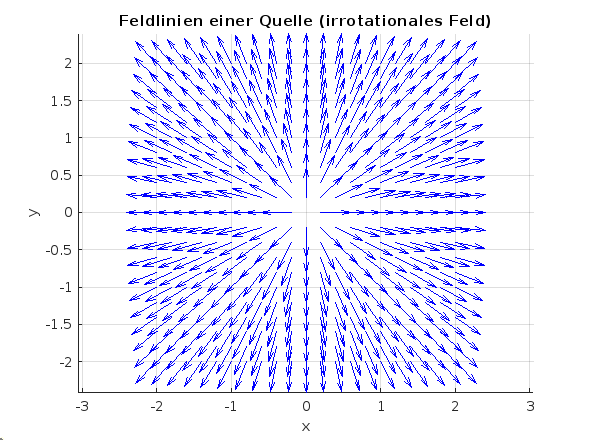
\includegraphics[width=0.8\textwidth]{papers/helmholtz/images/Quelle.png}
\caption{Quellenmuster im irrotationalen Feldanteil}
\label{fig:quelle}
\end{figure}
 
\begin{figure}
\centering
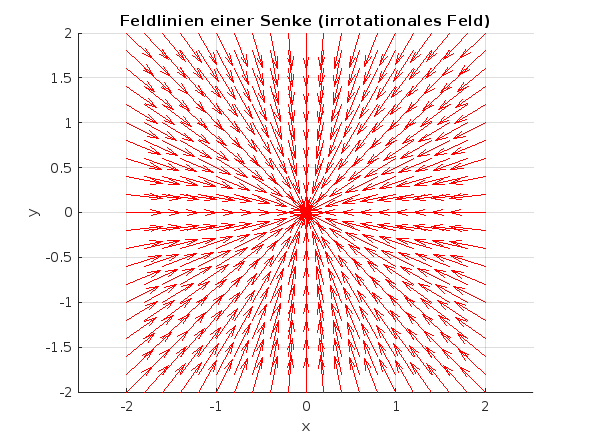
\includegraphics[width=0.8\textwidth]{papers/helmholtz/images/Senke.png}
\caption{Senkenmuster im irrotationalen Feldanteil}
\label{fig:senke}
\end{figure}
 
\item Der solenoidale Anteil bildet Wirbelfelder mit geschlossenen Feldlinien, ähnlich einem Magnetfeld.
\end{itemize}
  
\begin{figure}
\centering
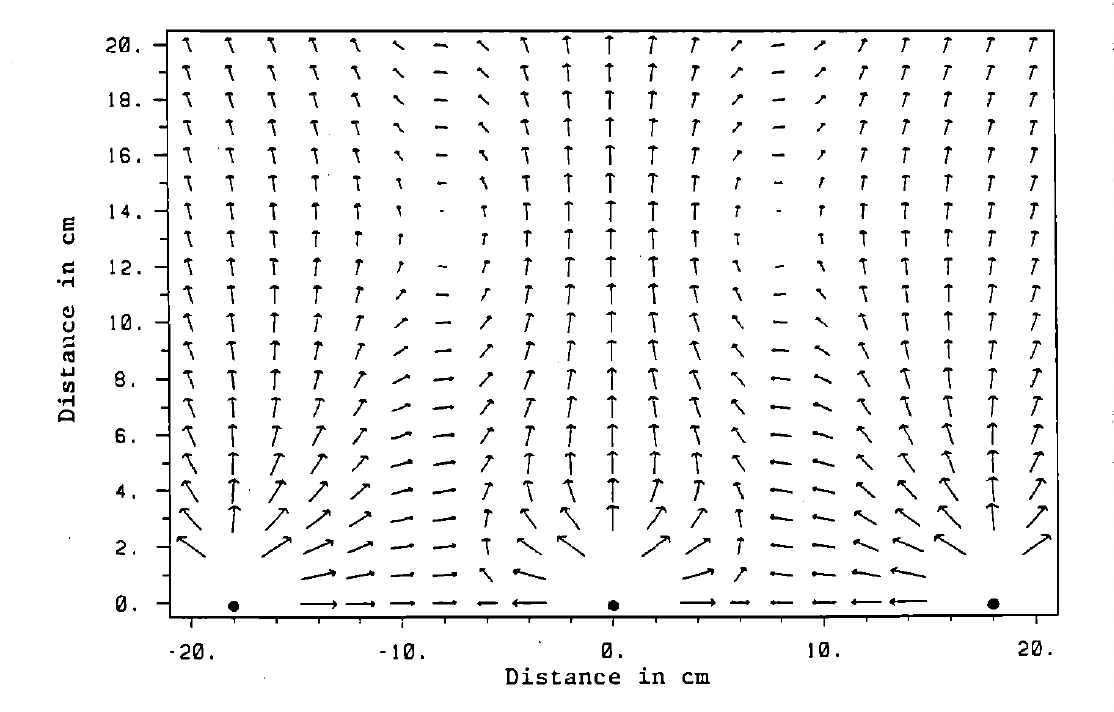
\includegraphics[scale=0.6]{papers/helmholtz/images/aktiveSchallintensitaet.png}
\caption{Visualisierung des aktiven Schallintensitätsfeldes für eine Anordnung von drei Punktquellen. Die Pfeile stellen die Vektoren der aktiven Intensität dar und zeigen die Richtung des zeitgemittelten Netto-Energieflusses. In der Nähe der Quellen ist die radial wegführende Energie zu erkennen, während in den Interferenzzonen komplexe Muster, einschliesslich der Bildung von Schallintensitätswirbeln, sichtbar werden (Abbildung aus \cite{helmholtz:paper}).}
\label{fig:aktive_intensitaet_3quellen}
\end{figure}
 
Die Visualisierung der Feldmuster erlaubt eine intuitive Interpretation von Schallfeldern:
 
\begin{itemize}
\item in Bereiche mit starker aktiver Intensität zeigen Energieausbreitung und -übertragung.
\item in Bereiche mit starker reaktiver Intensität zeigen Energieoszillation ohne Nettotransport, wie sie typischerweise im Nahfeld von Schallquellen oder bei stehenden Wellen auftritt.
\item Die räumliche Verteilung von Quellen, Senken und Wirbeln erlaubt Rückschlüsse auf die zugrundeliegenden Schallquellen und Reflexionsmuster. 

Abbildung \ref{fig:aktive_intensitaet_3quellen} verdeutlicht eindrücklich, wie die Interferenz von nur drei Quellen ausreicht, um solche komplexen Wirbelmuster zu erzeugen.
\end{itemize}
Diese Feldmuster sind besonders wichtig für die akustische Messtechnik, da sie eine visuelle Methode zur Identifikation von Schallquellen und zur Analyse von Energieflüssen in komplexen akustischen Feldern bieten.




